

\section{Data processing} \label{sec:M:dataProcessing}

The following two sections will cover the implementation of the filter used to prepare the EMG-signal and the extraction of features to represent the signal. Choices behind implemented methods builds on background knowledge acquired in \secref{sec:BG:dataProcessing}.

\subsection{Filtering of signal} \label{sub:M:filtering} 

As earlier mentioned in \subref{sub:BG:filtering}, due to the MYB specifications limiting the sample rate to 200 Hz and due to movement artefacts in the low-frequency spectrum, it would be resourceful to implement a bandpass filter to avoid a biased signal.
In the interest of representing the signal with its true properties a second order Butterworth bandpass filter has been implemented with cut-off frequencies at 10 Hz and 90 Hz. A filter steeper than second order was deselected due to a chosen trade-off between filter performance and computational performance, which is of great importance when doing real-time control. In \figref{fig:filt} is the result of the bandpass filter implementation shown. The unfiltered signal shows frequency components in low-frequency spectrum around 0-10 Hz and indicating frequency components at 100 Hz. Both ends of the spectrum have been attenuated limiting impact of artefacts. Furthermore is the presence of the build-in 50 Hz notch filter seen as explained in \subref{sub:BG:MYB}.     


\begin{figure}[H]                 
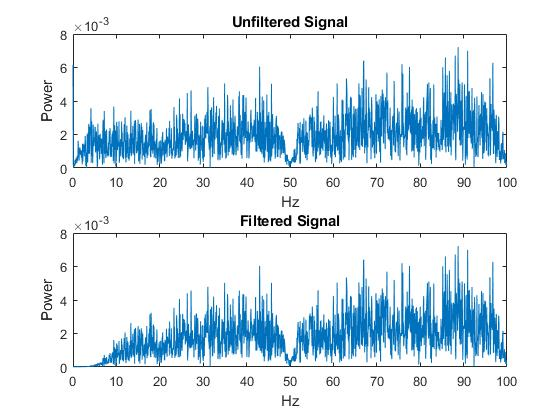
\includegraphics[width=.8\textwidth]{figures/pMethods/Filt}  
\caption{Frequency spectrum of a randomly selected EMG-recording showing the difference before an after implementing the bandpass filter. The unfiltered signal shows frequency components in low-frequency spectrum around 0-10 Hz and indicating frequency components at 100 Hz. The filtered signal shows reduction in the signal outside the cut-off frequencies.}
\label{fig:filt} 
\end{figure}

\subsection{Feature extraction} \label{sub:M:featureExtraction}

In \subref{sub:BG:featureExtraction} it was stated that when extracting features for real-time prosthesis control, features are extracted from segments of the signal called windows. This projects will for the feature extraction utilize a window size of 200 ms and a 50 \% overlap for all channels. This thereby gives the possibility of calculating and updating the feature values ten times a second, thus minimizing the update delay in the real-time user training and performance test.  

The features chosen to represent the information of movements contained in the signal is primarily based on recommendations from \cite{Donovan2017} where they found the optimal features for a real-time classification control scheme using the MYB. Donovan et al. \cite{Donovan2017} used so called space domain features along with the MYB and got a five percent higher accuracy than by using the well known Hudgins time domain features. A total of seven features, Mean Absolute Value (MAV), Mean Mean Absolute Value (MMAV), Scaled Mean Absolute Value (SMAV), Correlation Coefficient (CC), Mean Absolute Difference Normalized (MADN), Mean Absolute Difference Raw (MADR) and Scaled Mean Absolute Difference Raw (SMADR) were derived and the following section will explain the extraction of each. This project will use SMAV, CC, MADN and SMADR for the final classification to reduce redundancy, but all seven will be explained because some features are a combination of others. \cite{Donovan2017} Furthermore it has been chosen to extract the time domain feature of waveform length (WL) to represent frequency related information of the signal. The extraction of this feature will lastly be explained as well. 

MAV is a feature that primarily is affected by the force produces when making a contraction. MAV is extracted for each window and calculated for each of the $i^{th}$ channel. The extraction is expressed as:

\begin{equation} \label{eq:MAV}
MAV_i=\frac{\sum_{n=1}^{ws}|x_i[n]|}{ws}
\end{equation}
  
where $ws$ is the window size, the number of raw data points in that exact window. $x_i[n]$ is the $n^{th}$ raw data points from the $i^{th}$ channel.  

The mean MAV across all channels, MMAV, is used to remove dependency of movement intensity. MMAV is calculated by using the MAV of all channels for the current window, and is done as following: 

\begin{equation} \label{eq:MMAV}
MMAV=\frac{\sum_{i=1}^{8}MAV_i}{8}
\end{equation}

MMAV can be used to scale the MAV feature creating the SMAV feature. This feature should represent a non-dimensional relationship between channels. SMAV is simply calculated as:

\begin{equation} \label{eq:SMAV}
SMAV_i=\frac{MAV_i}{MMAV}
\end{equation}

As each of the eight EMG sensors in the MYB are located around the arm, they acquire signals from a mixture of sources. Also individual sources may affect multiple sensors depending on their size. Due to this a source measured by multiple sensors will effect their acquired signal correlation. An idea is therefore to calculate the correlation coefficient between each channel and its neighboring channel.  

\begin{equation} \label{eq:CC}
CC_i=\frac{\sum_{n=1}^{ws}X_i[n]X_{i+1}[n]}{ws}
\end{equation}

$X_i[n]$ is the $n^{th}$ normalized data point from channel $i$. When calculating CC the data from each window is normalized by subtracting its mean value from each raw data point, and afterwards divided by their standard deviation. 

Calculating CC can prove rather demanding in computational power due to the series og multiplication operations. Therefore Donovan et al. \cite{Donovan2017} proposed introducing a mean absolute difference-based feature of lower computational complexity which still characterizes the spatial relationship between channels. The MAD feature is normalized in the same way as CC, making up the MADN feature calculated as: 

\begin{equation} \label{eq:MADN}
MADN_i=\frac{\sum_{n=1}^{ws}|X_i[n]-X_{i+1}[n]|}{ws}
\end{equation}

If the normalization of the signal proves too demanding the feature can be calculated on the raw EMG-signal without the normalization. This makes up the MADR feature, calculated as:

\begin{equation} \label{eq:MADR}
MADR_i=\frac{\sum_{n=1}^{ws}|x_i[n]-x_{i+1}[n]|}{ws}
\end{equation}

As the SMAV feature the MAD feature can be scaled by MMAV to remove movement intensity dependency. SMADR is calculated for each channel by:

\begin{equation} \label{eq:MMADR}
SMADR_i=\frac{MADR_i}{MMAV}
\end{equation}


As stated in the beginning some of these features introduce redundancy, subsequently the features of SMAV, CC, MADN and SMADR are the ones used for classification. \cite{Donovan2017}

To further improve the decision foundation of the classifier it was proposed to include the time domain feature of WL calculated by: 

\begin{equation} \label{eq:WL}
WL_i=\sum_{n=1}^{N-1}|x_{i+1}[n]-x_i[n]|
\end{equation}

WL is a measure of the signal complexity by calculating the cumulative length for each channel \cite{Phiny2012}.




